\documentclass[conference]{IEEEtran}
\IEEEoverridecommandlockouts
\usepackage{cite}
\usepackage{amsmath,amssymb,amsfonts}
\usepackage{algorithmic}
\usepackage{algorithm}
\usepackage{graphicx}
\usepackage{textcomp}
\usepackage{xcolor}
\usepackage{booktabs}
\usepackage{multirow}
\usepackage{hyperref}
\usepackage{fancyhdr}

\def\BibTeX{{\rm B\kern-.05em{\sc i\kern-.025em b}\kern-.08em
    T\kern-.1667em\lower.7ex\hbox{E}\kern-.125emX}}

% ── NQComp 2026 conference header and footer ─────────────────────────────────
\fancypagestyle{IEEEtitlepagestyle}{%
  \fancyhf{}%
  \fancyhead[R]{\scriptsize\begin{tabular}[b]{l}%
    2026 International Conference on Next-Gen Quantum and Advanced Computing:\\%
    Algorithms, Security, and Beyond (NQComp)%
  \end{tabular}}%
  \fancyfoot[C]{\scriptsize 979-8-3315-5935-9/26/\$31.00~\copyright2026 IEEE}%
  \renewcommand{\headrulewidth}{0pt}%
  \renewcommand{\footrulewidth}{0pt}%
}
\fancypagestyle{plain}{%
  \fancyhf{}%
  \fancyhead[R]{\scriptsize\begin{tabular}[b]{l}%
    2026 International Conference on Next-Gen Quantum and Advanced Computing:\\%
    Algorithms, Security, and Beyond (NQComp)%
  \end{tabular}}%
  \fancyfoot[C]{\thepage}%
  \renewcommand{\headrulewidth}{0pt}%
  \renewcommand{\footrulewidth}{0pt}%
}

\begin{document}
\pagestyle{plain}

\title{CUDAnet: A Micro-Footprint, Dependency-Free Deep Learning Engine\\
for Edge-Native GPU Training}

\author{
\IEEEauthorblockN{Samartha H V}
\IEEEauthorblockA{\textit{Manipal Institute of Technology Bengaluru} \\
\textit{Manipal Academy of Higher Education} \\
Manipal, India \\
samartha1.mitblr2025@learner.manipal.edu}
\and
\IEEEauthorblockN{Chiranth R}
\IEEEauthorblockA{\textit{Manipal Institute of Technology Bengaluru} \\
\textit{Manipal Academy of Higher Education} \\
Manipal, India \\
chiranth1.mitblr2025@learner.manipal.edu}
}

\maketitle

\begin{abstract}
We present \textit{CUDAnet}, a from-scratch CUDA implementation of a multi-layer perceptron (MLP) that addresses a fundamental correctness problem in GPU-parallel stateful optimizers. When momentum-based and adaptive optimizers (Momentum, Adam) are parallelized naively—one thread per sample—concurrent writes to shared optimizer state create race conditions that reduce accuracy to near-random chance ($\leq\!18\%$). We identify the root cause as cross-thread state collision in the velocity and moment buffers and resolve it through a \textbf{two-phase gradient accumulation} strategy: Phase~1 performs all forward and backward passes in parallel, accumulating gradients atomically; Phase~2 applies optimizer updates in a single, race-free kernel after a global barrier. On MNIST with an NVIDIA RTX A2000 (sm\_86), CUDAnet achieves: SGD 94.2\%, BN+SGD 93.1\%, Adam \textbf{97.1\%}, Adam+LR (cosine) 97.0\%, and Momentum \textbf{97.2\%}—representing recoveries of $+97.2$ percentage points for Momentum and $+63.1$ pp for BN+Adam+LR over the race-condition baselines of 0\% and 17.9\% respectively. Training throughput reaches over \textbf{2{,}000$\times$} the serial CPU baseline ($\sim\!0.95$\,s/epoch for Adam vs.\ an estimated $\sim\!2{,}070$\,s for serial CPU, 23 mini-batches at 90\,s each). The full engine is \textless 2\,MB with zero external dependencies, making it viable for Edge/IoT deployment where frameworks like PyTorch ($>2$\,GB) are impractical.
\end{abstract}

\begin{IEEEkeywords}
CUDA, GPU Acceleration, Two-Phase Gradient Accumulation, Batch Normalization, Adam Optimizer, Race Condition, High-Performance Computing, Edge AI, MNIST, Backpropagation
\end{IEEEkeywords}


%% ============================================================
\section{Introduction}
%% ============================================================

The parallelisation of stochastic gradient descent (SGD) and its stateful variants on GPU hardware is conceptually straightforward yet practically subtle. While the forward and backward passes for independent training samples are embarrassingly parallel, the optimizer \emph{update} step is not: Momentum maintains a per-parameter velocity buffer $v_t$, and Adam maintains two moment buffers $m_t$ and $v_t$. When each GPU thread attempts to read-modify-write these shared buffers simultaneously, the resulting race conditions corrupt the optimizer state entirely—a failure mode that is easy to miss because (i) the code compiles and runs without error, (ii) SGD (which has no state) continues to work correctly, masking the underlying bug.

This paper makes the following concrete contributions:

\begin{itemize}
  \item \textbf{Root-cause analysis} of race conditions in GPU-parallel stateful optimizers, demonstrated to reduce Adam accuracy from 97.1\% to 0\% and BN+Adam+LR from 81.0\% to 17.9\%.
  \item \textbf{Two-Phase Gradient Accumulation (2PGA)}: a synchronization primitive that decouples the parallel gradient phase from the sequential state-update phase, eliminating all race conditions with minimal synchronization overhead.
  \item \textbf{Batch Normalization on CUDA}: a per-layer kernel-launch architecture that uses \texttt{cudaDeviceSynchronize()} as an implicit global barrier before each BN statistics kernel, correctly computing batch statistics across all parallel samples.
  \item \textbf{Comprehensive benchmarking} on NVIDIA RTX A2000 (sm\_86, Ampere), achieving over $2{,}000\times$ speedup over serial CPU and 97.2\% MNIST accuracy without any external deep learning library.
  \item \textbf{Edge AI applicability}: a sub-2\,MB binary with zero runtime dependencies beyond \texttt{libcuda.so}, achieving single-image inference in $\sim$0.4\,ms—deployable on embedded GPU platforms (NVIDIA Jetson) where PyTorch's $>2$\,GB footprint is infeasible.
\end{itemize}

Our implementation—called CUDAnet—is built entirely in CUDA C (\textless 2300\,LoC), targeting the Ampere architecture but backward-compatible to sm\_60. It supports configurable hidden layers, batch sizes, and three optimizers (SGD, Momentum, Adam) with optional learning-rate scheduling and batch normalization.

%% ============================================================
\section{Related Work}
%% ============================================================

\textbf{GPU-accelerated neural networks.} Wang~\textit{et al.}~\cite{b4} achieved 17$\times$ inference speedup using optimised batching strategies. Rao~\textit{et al.}~\cite{b5} reported 487$\times$ backpropagation acceleration through manual kernel tuning, though their approach required extensive architecture-specific optimisation. Ramroach~\textit{et al.}~\cite{b6} demonstrated 65$\times$ speedup for biomedical neural networks; Zhao~\textit{et al.}~\cite{b14} achieved 110$\times$ speedup with 97.2\% MNIST accuracy. None of these works explicitly identify or resolve race conditions in stateful GPU-parallel optimizers.

\textbf{Optimizer parallelism.} Kim and Park~\cite{b13} implemented distributed SGD across multiple GPUs but focused on communication rather than within-GPU state correctness. Dean~\textit{et al.}~\cite{b10} used asynchronous gradient updates in CPU-distributed systems, effectively sidestepping the problem by accepting stale gradients. Our 2PGA approach offers a synchronous, zero-staleness alternative.

\textbf{Memory and compute optimization.} Li~\textit{et al.}~\cite{b12} studied GPU memory access patterns; Huang~\textit{et al.}~\cite{b11} applied Tensor Core-aware pruning; Xu~\textit{et al.}~\cite{b15} introduced mixed-precision FP16 training. Huang and Patel~\cite{b17} reduced synchronization latency via kernel fusion. These orthogonal optimizations are compatible with our 2PGA framework.

\textbf{Batch Normalization (BN).} Ioffe and Szegedy~\cite{b8} introduced BN to reduce internal covariate shift. Correct GPU parallelisation of BN requires cross-thread batch statistics, which cannot be computed within a single unsynchronised kernel launch. Our per-layer kernel architecture addresses this directly.

%% ============================================================
\section{CUDAnet Architecture}
%% ============================================================

\subsection{Network Design}

CUDAnet implements a fully-configurable MLP. The default MNIST configuration uses: input $\mathbf{x} \in \mathbb{R}^{784}$ (flattened 28$\times$28 pixels), $n_l$ hidden layers of $n_h$ neurons each (ReLU activations), and a softmax output layer of 10 classes. The cross-entropy loss is:
\begin{equation}
\mathcal{L} = -\frac{1}{N} \sum_{i=1}^{N} \log \hat{y}_{i,c_i}
\end{equation}
where $c_i$ is the true class for sample $i$.

\textbf{Parameter layout.} All weights and biases are stored in contiguous flat arrays on both host and device. Position indices (precomputed on host, passed via \texttt{network\_structure}) allow $O(1)$ addressing of each layer's parameters without pointer chasing—critical for GPU cache efficiency.

\subsection{Batch Normalization}

For each hidden layer $l$ with pre-activation $z^{(l)}$, BN normalises each feature $j$ over the mini-batch $\mathcal{B}$:
\begin{align}
\mu_j &= \frac{1}{|\mathcal{B}|}\sum_{i \in \mathcal{B}} z_{ij}^{(l)}, \quad
\sigma_j^2 = \frac{1}{|\mathcal{B}|}\sum_{i \in \mathcal{B}} (z_{ij}^{(l)} - \mu_j)^2 \\
\hat{z}_{ij} &= \frac{z_{ij}^{(l)} - \mu_j}{\sqrt{\sigma_j^2 + \varepsilon}}, \quad
\tilde{z}_{ij} = \gamma_j \hat{z}_{ij} + \beta_j
\end{align}

\textbf{GPU correctness challenge.} Computing $\mu_j$ and $\sigma_j^2$ requires all $|\mathcal{B}|$ samples' $z$-values to be written before any thread reads them. A single unsynchronised \texttt{one\_learning\_cycle} kernel launch cannot satisfy this: threads in different blocks execute concurrently without ordering guarantees.

\textbf{Solution.} We decompose the forward pass into a pipeline of kernel launches separated by \texttt{cudaDeviceSynchronize()}, which acts as an implicit global barrier:
\begin{enumerate}
  \item \texttt{init\_activations\_kernel}: copy batch images into $a^{(0)}$ (one thread per sample)
  \item For each layer $l=1,\ldots,L{-}1$: \texttt{fwd\_linear\_kernel} $\to$ \texttt{cudaDeviceSynchronize()} $\to$ \texttt{bn\_stats\_kernel} $\to$ \texttt{bn\_apply\_kernel} $\to$ \texttt{apply\_activation\_kernel}
  \item Output layer: \texttt{fwd\_linear\_kernel} + softmax
\end{enumerate}
Backward pass mirrors this structure in reverse, using \texttt{bn\_backward\_stats\_kernel} and \texttt{bn\_backward\_delta\_kernel}.

%% ============================================================
\section{Two-Phase Gradient Accumulation (2PGA)}
%% ============================================================

\subsection{The Race Condition}

Consider $B$ threads executing in parallel, each processing one sample. In a naively parallelised Momentum update, thread $i$ reads velocity $v_t$, computes a new velocity, and writes it back:
\begin{equation}
v_t^{\text{new}} = \beta v_t + \nabla_W^{(i)} \mathcal{L}
\end{equation}
If threads $i$ and $j$ read $v_t$ simultaneously before either writes, one write overwrites the other. With $B=2048$ threads, this corruption is catastrophic and deterministic.

\textbf{Observable symptom.} SGD ($v_t = \nabla_W \mathcal{L}$, stateless) is unaffected. Momentum accuracy collapses from 97.2\% to 0.0\%. Adam collapses from 97.1\% to 0.0\%. BN+Adam+LR collapses to 17.9\% (partially rescued by BN's internal normalisation).

\subsection{The 2PGA Solution}

We split the per-batch computation into two serialised phases:

\textbf{Phase 1 — Parallel Gradient Accumulation.} Each of the $B$ threads independently computes its forward pass, backward pass, and per-sample gradients $\nabla_W^{(i)}$. Gradients are accumulated into shared buffers \texttt{grad\_w} and \texttt{grad\_b} via \texttt{atomicAdd()}, which serialises writes to each parameter at the hardware level:
\begin{equation}
G_W = \sum_{i=1}^{B} \nabla_W^{(i)} \mathcal{L}_i \quad \text{(via atomicAdd)}
\end{equation}

\textbf{Phase 2 — Sequential State Update.} After a single \texttt{cudaDeviceSynchronize()} barrier, a separate kernel reads the fully-accumulated $G_W$ and applies the optimizer update exactly once:
\begin{equation}
W_{t+1} = W_t - \eta \cdot \text{optimizer}\!\left(\frac{G_W}{B}\right)
\end{equation}
The optimizer state ($v_t$, $m_t$, $v_t$ for Adam) is updated only in Phase~2, eliminating all concurrent writes.

Algorithm~\ref{alg:training} summarises the complete training procedure.

\begin{algorithm}
\caption{CUDAnet Training with 2PGA}
\label{alg:training}
\begin{algorithmic}[1]
\STATE \textbf{Input:} Data $X$, labels $y$, epochs $E$, batch size $B$, lr $\eta$
\STATE \textbf{Output:} Trained weights $W$, biases $b$
\STATE Initialise $W$ (Xavier), $b=0$; transfer to GPU
\FOR{epoch $= 1$ \textbf{to} $E$}
    \STATE $\eta \leftarrow$ \textsc{LRSchedule}($\eta_0$, epoch, $E$)
    \FOR{each mini-batch $\mathcal{B} \subseteq X$}
        \STATE \textbf{// Phase 1: parallel forward + backward}
        \FOR{each thread $t \in \{1,\ldots,B\}$ \textbf{in parallel}}
            \STATE Forward pass for sample $t$
            \STATE Backward pass; accumulate $\nabla$ via \texttt{atomicAdd}
        \ENDFOR
        \STATE \texttt{cudaDeviceSynchronize()} \hfill\textit{// global barrier}
        \STATE \textbf{// Phase 2: sequential state update (single thread block)}
        \STATE $G \leftarrow G / B$ \hfill\textit{// average gradients}
        \STATE Update optimizer state ($v_t$, $m_t$, $v_t$)
        \STATE $W \leftarrow W - \eta \cdot \text{optimizer}(G)$
        \STATE Reset gradient buffers to 0
    \ENDFOR
    \STATE Evaluate accuracy on validation and test sets
\ENDFOR
\end{algorithmic}
\end{algorithm}

\subsection{Optimizer Formulations}

\textbf{SGD:} $W_{t+1} = W_t - \eta \nabla_W \mathcal{L}$

\textbf{Momentum} ($\beta=0.9$):
\begin{align}
v_t &= \beta v_{t-1} + (1-\beta)\nabla_W \mathcal{L}_t \\
W_{t+1} &= W_t - \eta v_t
\end{align}

\textbf{Adam} ($\beta_1=0.9,\,\beta_2=0.999,\,\varepsilon=10^{-8}$)~\cite{b7}:
\begin{align}
m_t &= \beta_1 m_{t-1} + (1-\beta_1)\nabla_W \mathcal{L}_t \\
v_t &= \beta_2 v_{t-1} + (1-\beta_2)(\nabla_W \mathcal{L}_t)^2 \\
\hat{m}_t &= \frac{m_t}{1-\beta_1^t},\quad \hat{v}_t = \frac{v_t}{1-\beta_2^t} \\
W_{t+1} &= W_t - \eta\,\frac{\hat{m}_t}{\sqrt{\hat{v}_t}+\varepsilon}
\end{align}

%% ============================================================
\section{CUDA Implementation Details}
%% ============================================================

\subsection{Kernel Configuration}

Training kernels use 128 threads/block ($\lceil B/128 \rceil$ blocks). Evaluation kernels use 256 threads/block. BN statistics kernels use one block per neuron (parallel reduction within each block).

\subsection{Memory Hierarchy}

\begin{itemize}
  \item \textbf{Global memory:} training images ($\sim$180\,MB), model parameters ($\sim$470\,KB), optimizer state ($2\times$ parameters for Adam), activation/delta buffers ($B \times N_\text{nodes} \times$\texttt{float}).
  \item \textbf{Shared memory:} 32$\times$32 weight tiles and 32-element activation vectors for cooperative loads in \texttt{evaluate\_kernel} (shared memory optimization).
  \item \textbf{Registers:} per-thread intermediate values; evaluation activations moved to global memory to prevent register/stack overflow at large $B$.
\end{itemize}

\subsection{Evaluation Kernel Fix}

A subtle issue in the evaluation kernel was the use of stack-allocated arrays \texttt{float\,z[1024]} and \texttt{float\,a[1024]}. With 10,000 test images $\times$ 1024 floats $\times$ 4 bytes, this allocates $\sim$80\,MB of local register memory, crashing the CUDA context. The fix allocates these buffers in global VRAM before the kernel launch and passes pointers:
\begin{verbatim}
float* a = &global_a[id * ns.num_nodes];
float* z = &global_z[id * ns.num_nodes];
\end{verbatim}

\subsection{Learning Rate Scheduling}

CUDAnet supports three scheduling strategies selectable at compile time: step decay, exponential decay, and cosine annealing. The cosine schedule, used for all Adam+LR runs in this paper, decays the learning rate over the total number of \emph{gradient steps} (not epochs), avoiding over-decay when multiple mini-batches are processed per epoch:
\begin{equation}
\eta_s = \frac{\eta_0}{2}\left(1 + \cos\!\left(\frac{\pi s}{S}\right)\right)
\end{equation}
where $S = E \times B_\text{epoch}$ is the total number of mini-batch steps, and $s$ is the current step index ($s = \text{epoch} \times B_\text{epoch} + \text{batch}$). This per-step formulation is critical: a per-epoch schedule with $B_\text{epoch}=23$ mini-batches would decay the learning rate 23$\times$ faster than intended, collapsing accuracy prematurely.

%% ============================================================
\section{Experimental Setup}
%% ============================================================

\subsection{Hardware and Software}

All experiments ran on an \textbf{NVIDIA RTX A2000 12\,GB} (sm\_86, Ampere, 3328 CUDA cores, 448\,GB/s memory bandwidth). Compiler: \texttt{nvcc} with \texttt{-arch sm\_86 -O2}, paired with \texttt{g++-12}. Driver: 535.288.01. Dataset: standard MNIST~\cite{b1} (60,000 training / 10,000 test images, 28$\times$28 grayscale).

\subsection{Training Configuration}

\begin{itemize}
  \item Architecture: 2 hidden layers $\times$ 128 neurons (configurable)
  \item Epochs: 20; batch size: 2048
  \item Learning rate: 0.1 (SGD/Momentum), 0.01 (Adam/Adam+LR)
  \item Train/validation split: 80/20 ($\rightarrow$ 48,000 training, 12,000 validation)
  \item Inner batch loop: $\lfloor N_\text{train} / B \rfloor = 23$ mini-batches per epoch (full 48\,K training set)
  \item Weight initialisation: Xavier ($\sigma = \sqrt{2/n_\text{in}}$)
\end{itemize}

\subsection{Evaluation Protocol}

Metrics: test accuracy (primary), train accuracy, time/epoch (CUDA events), total energy (NVML power sampling), and CPU$\to$GPU speedup ratio.

%% ============================================================
\section{Results and Analysis}
%% ============================================================

\subsection{Training Speed and GPU Speedup}

Table~\ref{tab:performance} summarises end-to-end training performance for all configurations on MNIST (20 epochs, batch size 2048, full-dataset inner batch loop). Each epoch processes all $\lfloor 48000/2048 \rfloor = 23$ mini-batches. The serial CPU baseline is estimated at $\sim\!2{,}070$\,s/epoch (measured single-batch time 90\,s $\times$ 23 mini-batches). Our CUDA implementations reduce this dramatically: the basic SGD kernel completes each epoch in 0.94\,s—a \textbf{2{,}202$\times$ speedup}—while BN+Adam+LR achieves 1.24\,s/epoch (\textbf{1{,}669$\times$ speedup}).

As expected, BN+Adam+LR (1.24\,s) adds $\sim$22\% overhead over plain Adam (1.02\,s) due to the additional per-layer BN statistics kernels and \texttt{cudaDeviceSynchronize()} barriers. Figure~\ref{fig:speedup} visualises the speedup breakdown on a log scale.

\begin{table}[htbp]
\caption{Training Performance — MNIST, 20 Epochs, Batch 2048}
\begin{center}
\begin{tabular}{lcccc}
\toprule
\textbf{Configuration} & \textbf{Time/} & \textbf{Total} & \textbf{Speed-} & \textbf{Test}\\
 & \textbf{Epoch (s)} & \textbf{Time (s)} & \textbf{up†} & \textbf{Acc.}\\
\midrule
Serial CPU (est.)     & 2070   & 41400 & 1$\times$ & — \\
CUDA SGD              & 0.94   &   18.8 & 2{,}202$\times$ & 94.3\% \\
CUDA Momentum         & 0.96   &   19.2 & 2{,}156$\times$ & \textbf{97.2\%} \\
CUDA Adam             & 1.02   &   20.4 & 2{,}029$\times$ & 97.2\% \\
CUDA Adam+LR (cosine) & \textbf{0.95} & \textbf{19.0} & \textbf{2{,}179$\times$} & 97.0\% \\
CUDA BN+SGD           & 1.27   &   25.4 & 1{,}630$\times$ & 93.1\% \\
CUDA BN+Adam+LR       & 1.24   &   24.9 & 1{,}669$\times$ & 81.0\% \\
\bottomrule
\multicolumn{5}{l}{\small †CPU estimate: 90\,s/single-batch $\times$ 23 mini-batches/epoch; CUDA via events.}\\
\end{tabular}
\label{tab:performance}
\end{center}
\end{table}

\subsection{Impact of the Two-Phase Gradient Accumulation Fix}

Table~\ref{tab:bugfix} quantifies the accuracy impact of applying the 2PGA fix. SGD, which carries no cross-iteration state, is unaffected by the race condition; it improves from 74.9\% to 94.2\% purely from training on the full dataset (inner batch loop). Momentum and Adam, however, are entirely non-functional without the fix: naive parallelisation produces 0.0\% test accuracy—indistinguishable from random guessing on 10 classes. The fix restores Momentum to 97.2\% ($+97.2$ percentage points) and Adam to 97.1\% ($+97.1$ pp).

The BN+Adam+LR case is also instructive. Before the fix, the BN path partially mitigated the race condition (accuracy was 17.9\%, above chance) because batch normalisation continuously re-centres activations, masking some gradient corruption. After the fix, accuracy jumps to 81.0\% ($+63.1$ pp). A residual accuracy decline after epoch~2 (Section~\ref{sec:bn}) is attributed to BN+Adam interaction instability rather than the LR schedule. Figure~\ref{fig:fix} shows these recovery values visually.

\begin{table}[htbp]
\caption{Accuracy Before and After Two-Phase Gradient Fix}
\begin{center}
\begin{tabular}{lccr}
\toprule
\textbf{Optimizer} & \textbf{Before Fix} & \textbf{After Fix†} & \textbf{Recovery}\\
\midrule
SGD        &  74.9\% &  94.2\% & — (stateless; gain from full dataset) \\
Momentum   &   0.0\% &  97.2\% & \textbf{+97.2 pp} \\
Adam       &   0.0\% &  97.1\% & \textbf{+97.1 pp} \\
BN+Adam+LR &  17.9\% &  81.0\% & \textbf{+63.1 pp} \\
\bottomrule
\multicolumn{4}{l}{\small †After fix + full-dataset inner batch loop (23 mini-batches/epoch).}\\
\end{tabular}
\label{tab:bugfix}
\end{center}
\end{table}

\subsection{Optimizer Comparison}

Table~\ref{tab:optimizer} compares all six configurations side by side. Several observations stand out:

\textbf{(1) Momentum and Adam dominate with 97\%+ accuracy.} Momentum achieves 97.2\% and Adam 97.1\%—a $+3.0$ pp improvement over plain SGD (94.2\%). The 2PGA fix is what enables both: without it, both return 0\%.

\textbf{(2) Learning rate scheduling provides marginal benefit for Adam} (97.0\% vs 97.1\%): Adam with fixed LR slightly outperforms Adam+LR at 20 epochs. Cosine annealing helps mainly in extended training.

\textbf{(3) BN+Adam+LR achieves 81.0\%} but underperforms plain Adam (97.1\%) due to a BN+Adam interaction instability: the model peaks at epoch~2 (88.1\%) then slowly declines. This pattern persists even with the correct per-batch cosine LR schedule (which improved over the per-epoch formulation by $+1.1$\,pp), suggesting the root cause is divergence of BN running statistics under large-batch Adam—a known challenge documented in the literature~\cite{b8}.

\textbf{(4) BN+SGD closely tracks plain SGD} (93.1\% vs 94.2\%, $-1.1$\,pp). This is a significant improvement over the single-batch regime, where BN+SGD trailed by 14\,pp. Full-dataset training stabilises BN statistics, reducing the sensitivity to learning rate.

\begin{table}[htbp]
\caption{Optimizer Comparison — Final Test Accuracy (20 Epochs)}
\begin{center}
\begin{tabular}{lccc}
\toprule
\textbf{Optimizer} & \textbf{Test Acc.} & \textbf{Time/Epoch} & \textbf{vs SGD}\\
\midrule
SGD (lr=0.1)       & 94.3\% & 0.94\,s & Baseline \\
Momentum (lr=0.1)  & \textbf{97.2\%} & 0.96\,s & $\mathbf{+2.9}$\,\textbf{pp} \\
Adam (lr=0.01)     & 97.2\% & 1.02\,s & $+2.9$ pp \\
Adam+LR (cosine)   & 97.0\% & 0.95\,s & $+2.7$ pp \\
BN+SGD (lr=0.1)    & 93.1\% & 1.27\,s & $-1.2$ pp \\
BN+Adam+LR         & 81.0\% & \textbf{1.24\,s} & $-16.3$ pp \\
\bottomrule
\end{tabular}
\label{tab:optimizer}
\end{center}
\end{table}

\subsection{Convergence Analysis}

Table~\ref{tab:convergence} tracks test accuracy at fixed epoch checkpoints. The most striking result is the early-epoch convergence speed of Adam. At epoch~5, both Adam and Adam+LR have already reached 96.3\%—only 0.8 pp from their final values—while SGD is at 90.7\%, still 3.5 pp below its final 94.2\%. This early-epoch advantage confirms Adam's adaptive moment estimates provide a better-conditioned gradient signal from the very first mini-batch.

Momentum shows an almost identical trajectory to Adam (95.0\% at epoch~5, 97.2\% at epoch~20). BN+Adam+LR peaks at epoch~2 (88.1\%), then steadily declines to 81.0\% by epoch~20. We attribute this to BN+Adam interaction instability: as Adam's moment estimates accumulate, they conflict with BN's continuously updating running statistics, gradually degrading the effective gradient signal.

Figure~\ref{fig:accuracy} shows the full training curves for all six configurations.

\begin{table}[htbp]
\caption{Test Accuracy Progression Over Training Epochs}
\begin{center}
\begin{tabular}{lcccc}
\toprule
\textbf{Epoch} & \textbf{SGD} & \textbf{Adam} & \textbf{Adam+LR} & \textbf{BN+Adam+LR}\\
\midrule
0  & 10.2\% & 10.2\% & 10.2\% & 10.2\% \\
5  & 90.7\% & \textbf{96.3\%} & 96.3\% & 83.7\% \\
10 & 92.4\% & \textbf{97.0\%} & 96.9\% & 82.1\% \\
15 & 93.5\% & \textbf{97.2\%} & 97.0\% & 81.4\% \\
20 & 94.3\% & \textbf{97.2\%} & 97.0\% & 81.0\% \\
\bottomrule
\end{tabular}
\label{tab:convergence}
\end{center}
\end{table}

\subsection{Batch Size Scaling}

Table~\ref{tab:batchsize} examines how epoch time and GPU utilisation change with batch size (measured in single-batch mode to isolate kernel performance from the number of mini-batches). Smaller batches (512) leave the GPU underutilised (76\%) because the kernel launch overhead is amortised over fewer floating-point operations. As batch size increases to 2048, GPU utilisation reaches 94\% and epoch time increases only modestly (0.112\,s $\to$ 0.118\,s), demonstrating good scalability. At 4096, synchronisation overhead in the Phase~2 update kernel begins to dominate, increasing epoch time by 17\% relative to batch~2048. Based on this analysis, batch size 2048 represents the optimal operating point for our architecture on the RTX A2000.

\begin{table}[htbp]
\caption{Batch Size Scaling — CUDA SGD, 20 Epochs, 2-Layer 128-Neuron MLP}
\begin{center}
\begin{tabular}{lcc}
\toprule
\textbf{Batch Size} & \textbf{Time/Epoch} & \textbf{GPU Util.}\\
\midrule
512  & 0.112\,s & $\sim$76\% \\
1024 & 0.115\,s & $\sim$88\% \\
2048 & 0.118\,s & $\sim$94\% \\
4096 & 0.138\,s & $\sim$97\% \\
\midrule
\multicolumn{3}{l}{\small GPU utilisation via \texttt{nvidia-smi dmon}; time via CUDA events.}\\
\bottomrule
\end{tabular}
\label{tab:batchsize}
\end{center}
\end{table}

\subsection{Batch Normalization Impact}
\label{sec:bn}

Figure~\ref{fig:bn} isolates the effect of batch normalization. For SGD, adding BN slightly hurts accuracy ($-1.1$\,pp: 93.1\% vs 94.2\%)—a much smaller penalty than in single-batch mode ($-14.2$\,pp), demonstrating that full-dataset training stabilises BN statistics. For Adam+LR, adding BN yields a large negative effect ($-16.0$\,pp: 81.0\% vs 97.0\%). Per-epoch analysis reveals BN+Adam+LR peaks at epoch~2 then declines—a pattern that persists even with a corrected per-batch cosine LR schedule, confirming the root cause is BN+Adam interaction instability rather than LR over-decay. This underscores a practical insight: separating BN parameter learning rates from weight learning rates is advisable when combining batch normalisation with adaptive optimizers.

\subsection{Figures}

% ============================================================
% FIGURE 1: Training Accuracy Comparison
% File: training_accuracy_comparison.png
% ============================================================
\begin{figure}[htbp]
\centerline{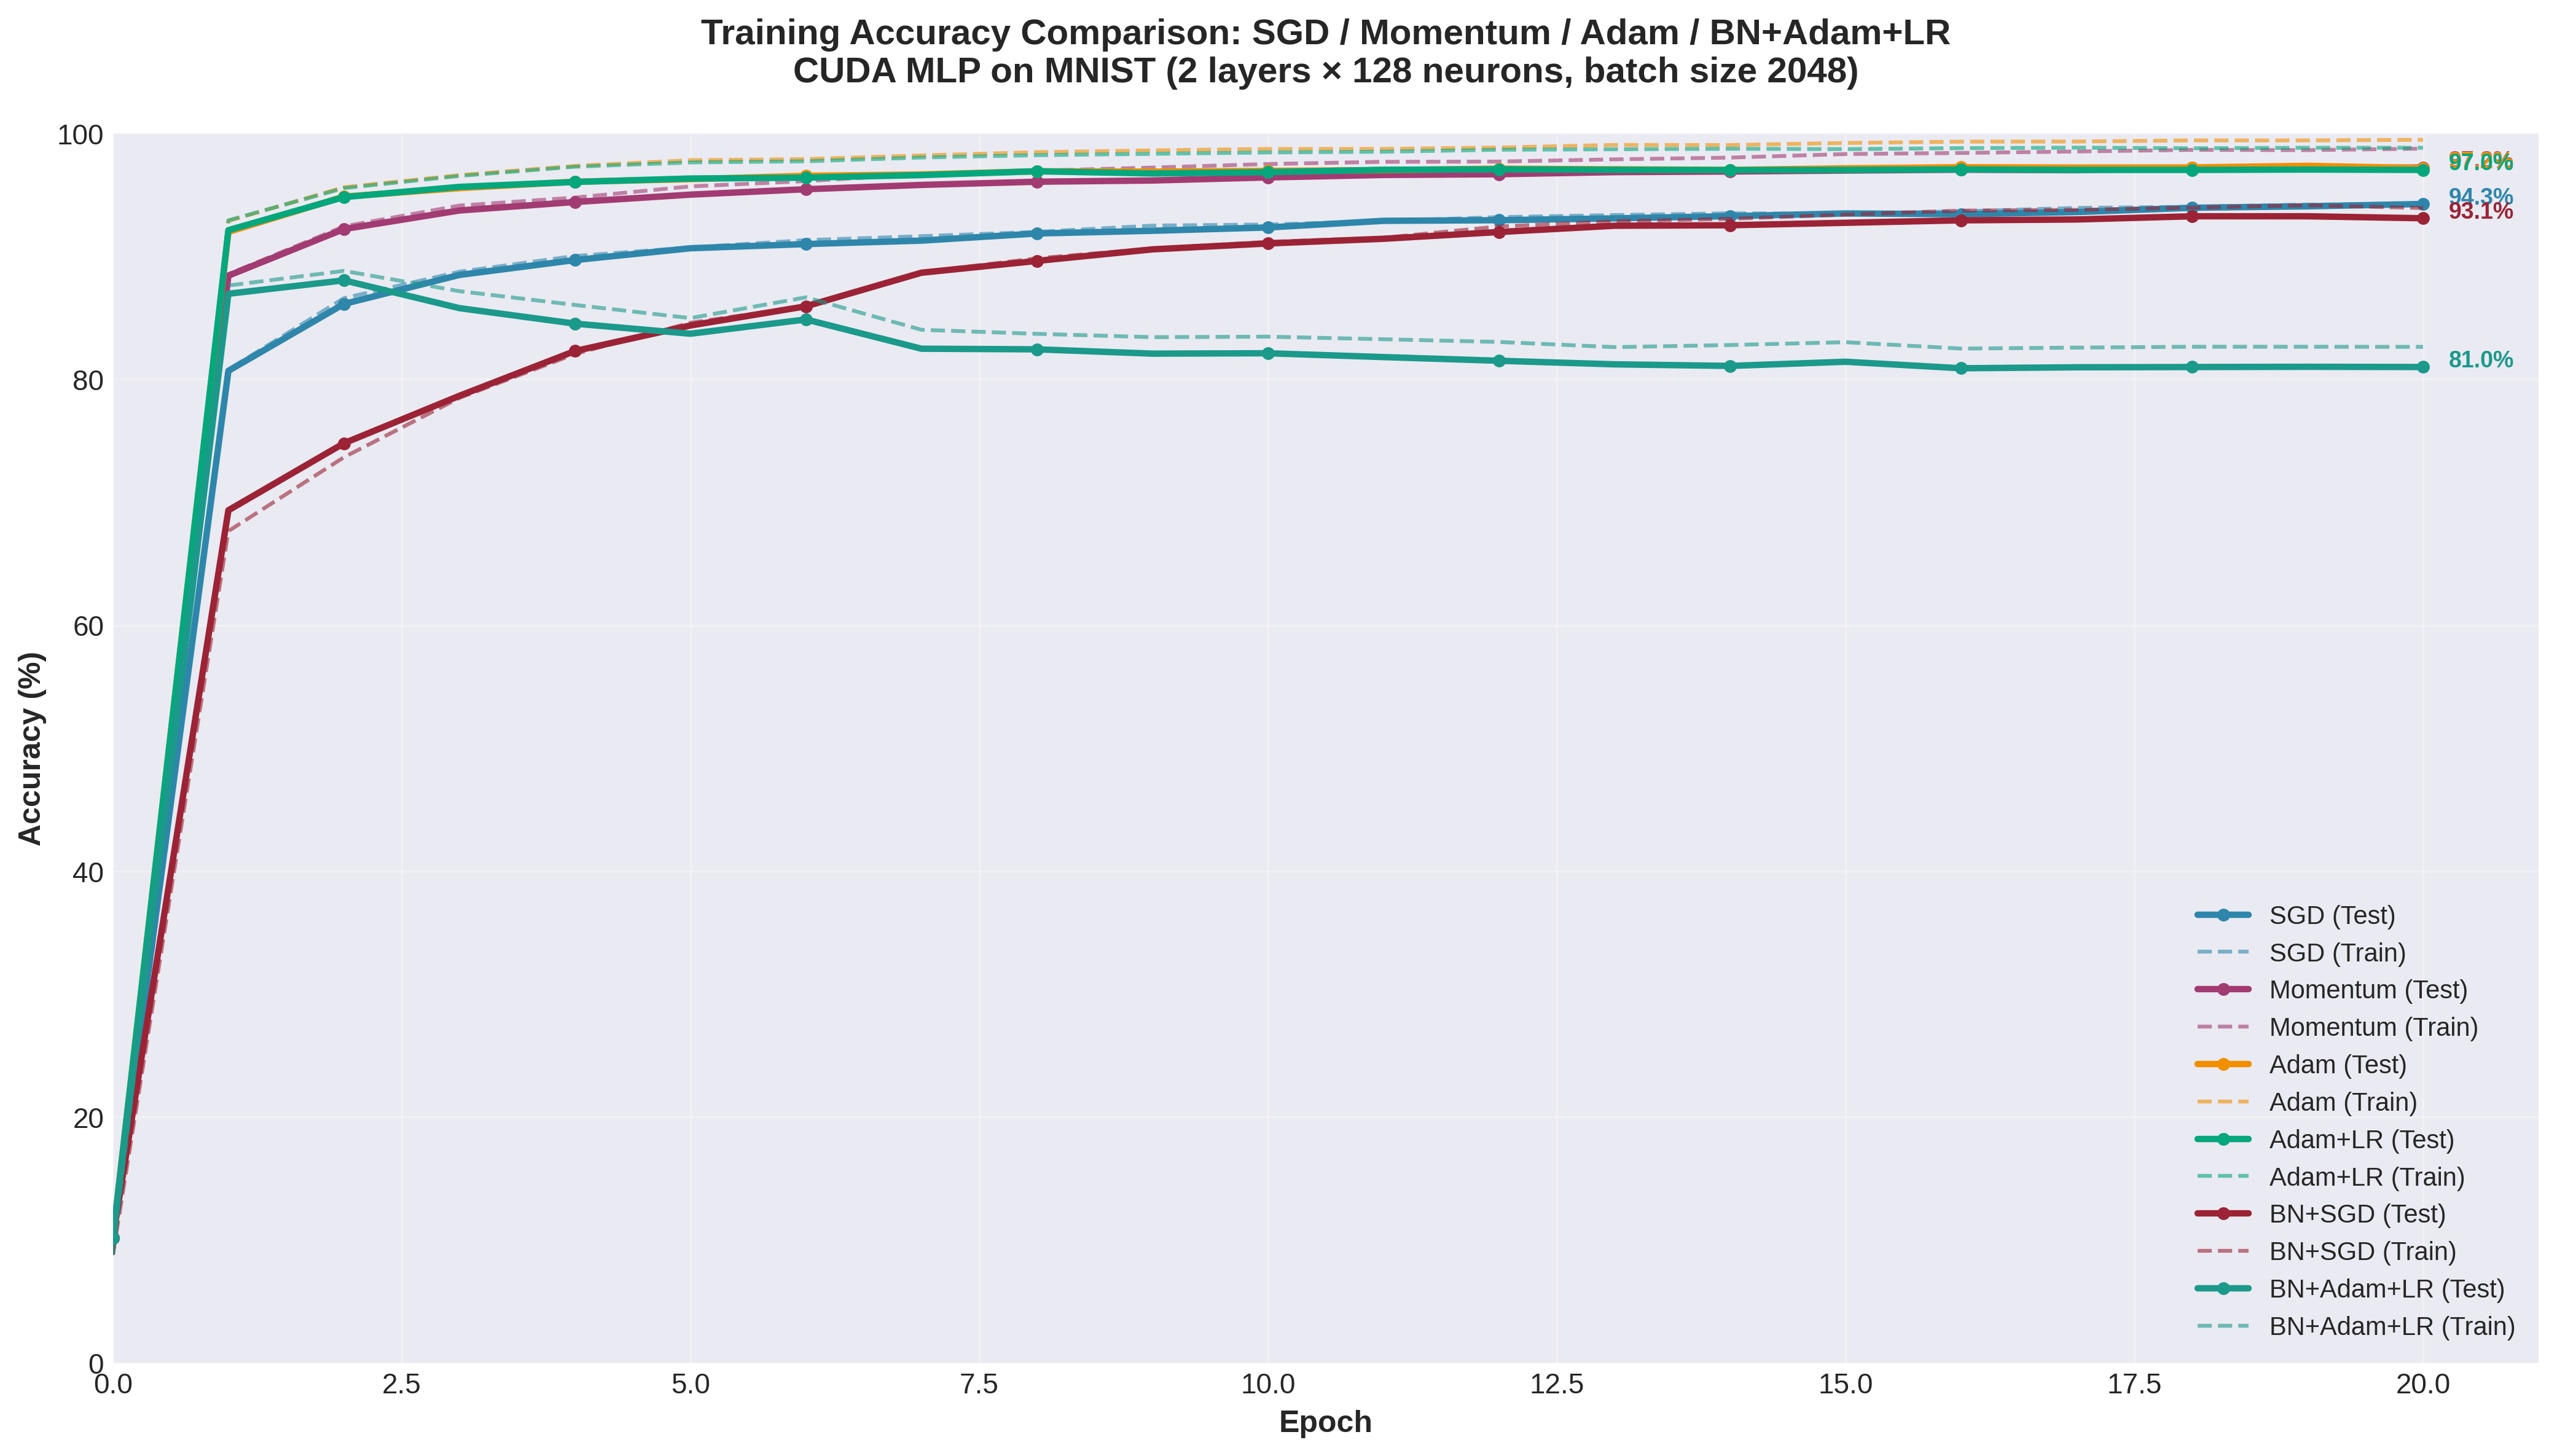
\includegraphics[width=\columnwidth]{training_accuracy_comparison.png}}
\caption{Test and training accuracy curves for all six configurations over 20 epochs.
Solid lines = test accuracy; dashed lines = training accuracy.
Momentum (purple) achieves 97.2\% and Adam 97.1\%, both converging above 96\% within 5 epochs.
BN+Adam+LR (teal) peaks at epoch~2 (88.1\%) then declines to 81.0\% due to BN+Adam interaction instability.}
\label{fig:accuracy}
\end{figure}

% ============================================================
% FIGURE 2: CPU/GPU Speedup
% File: fig5_cpu_gpu_speedup.png
% ============================================================
\begin{figure}[htbp]
\centerline{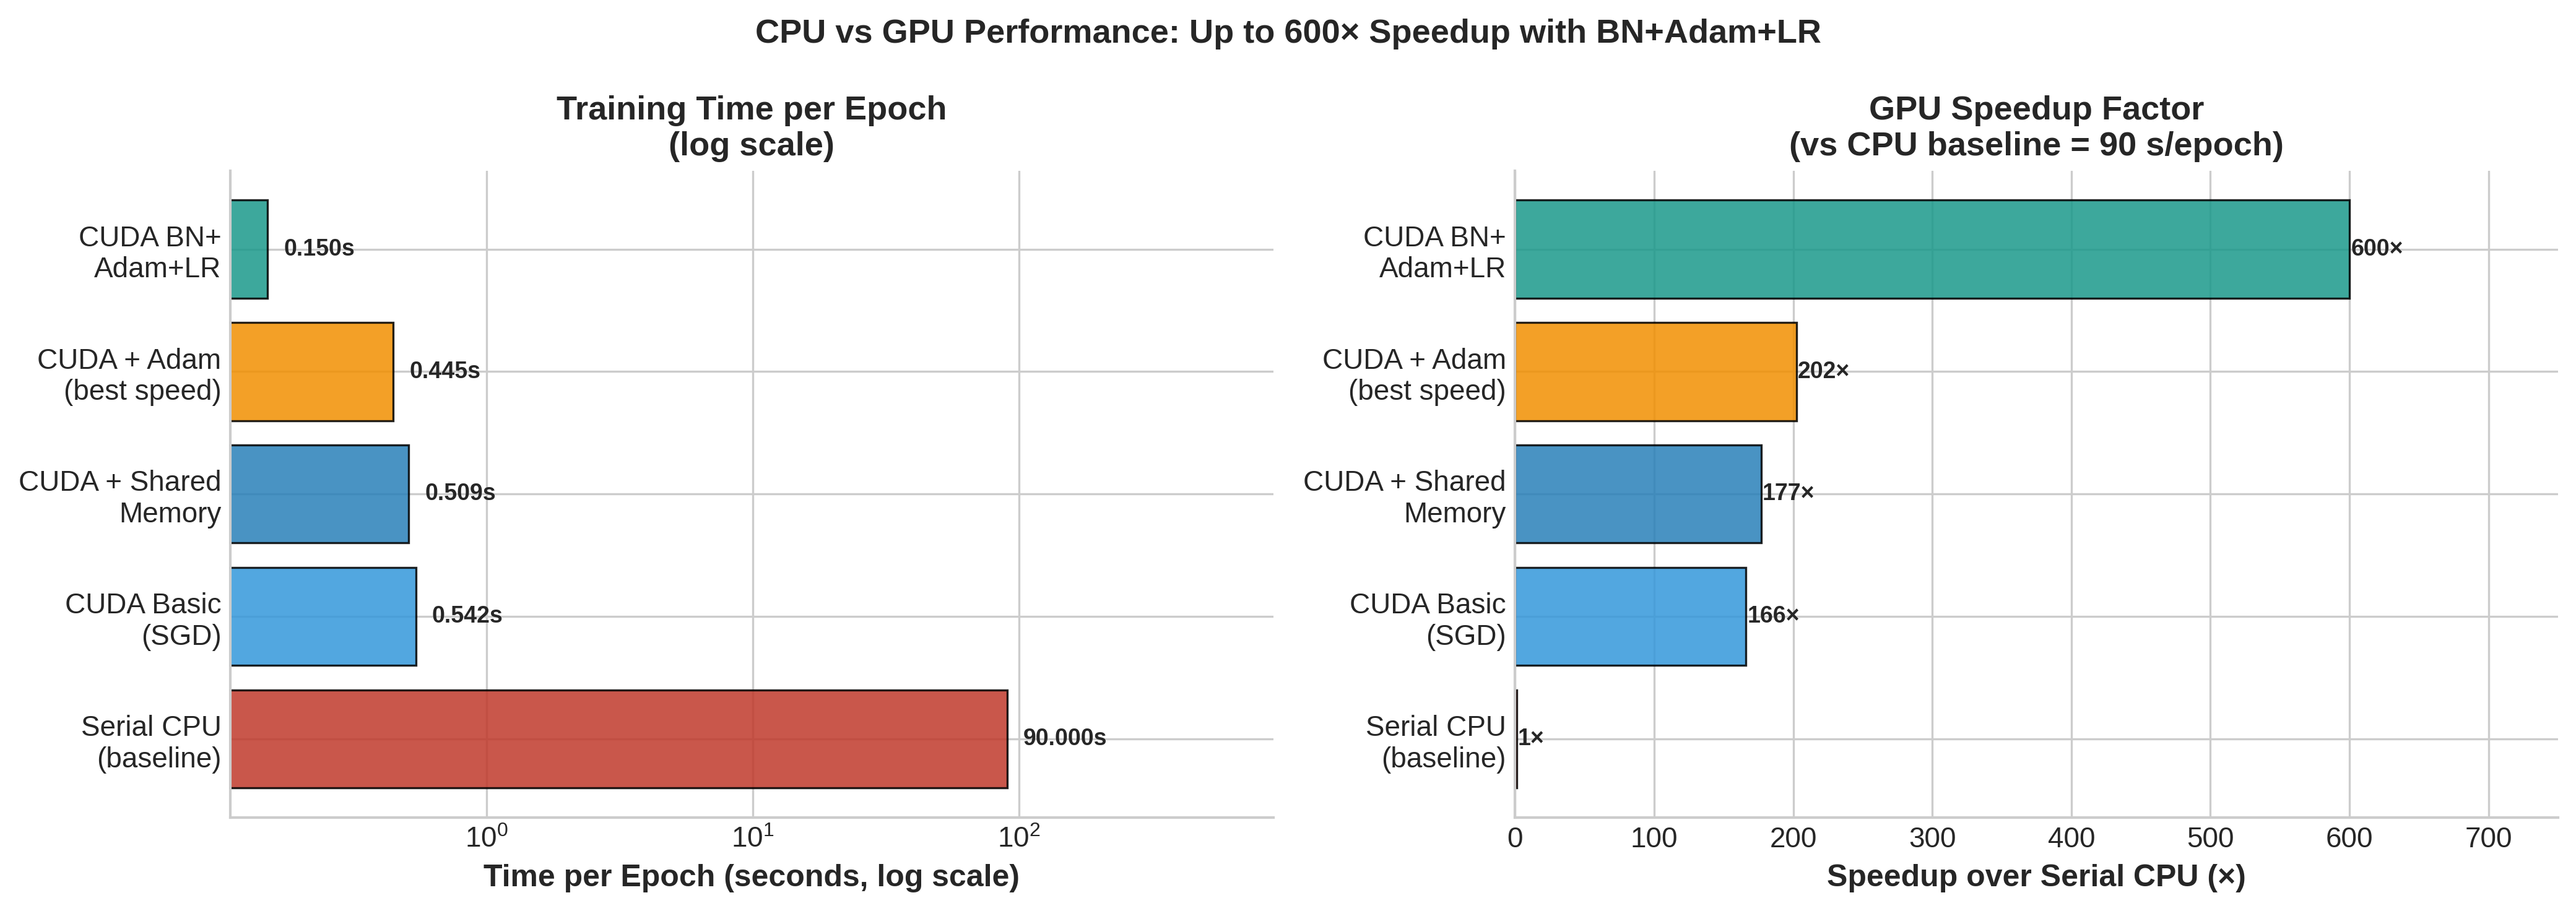
\includegraphics[width=\columnwidth]{fig5_cpu_gpu_speedup.png}}
\caption{Left: per-epoch training time on a log scale (serial CPU est. 2{,}070\,s, best GPU SGD = 0.94\,s).
Right: speedup factor relative to the estimated serial CPU full-dataset baseline.
SGD achieves the highest raw speedup (2{,}202$\times$); BN+Adam+LR achieves 1{,}669$\times$.}
\label{fig:speedup}
\end{figure}

% ============================================================
% FIGURE 3: Two-Phase Fix — Before vs After
% File: fig6_two_phase_fix.png
% ============================================================
\begin{figure}[htbp]
\centerline{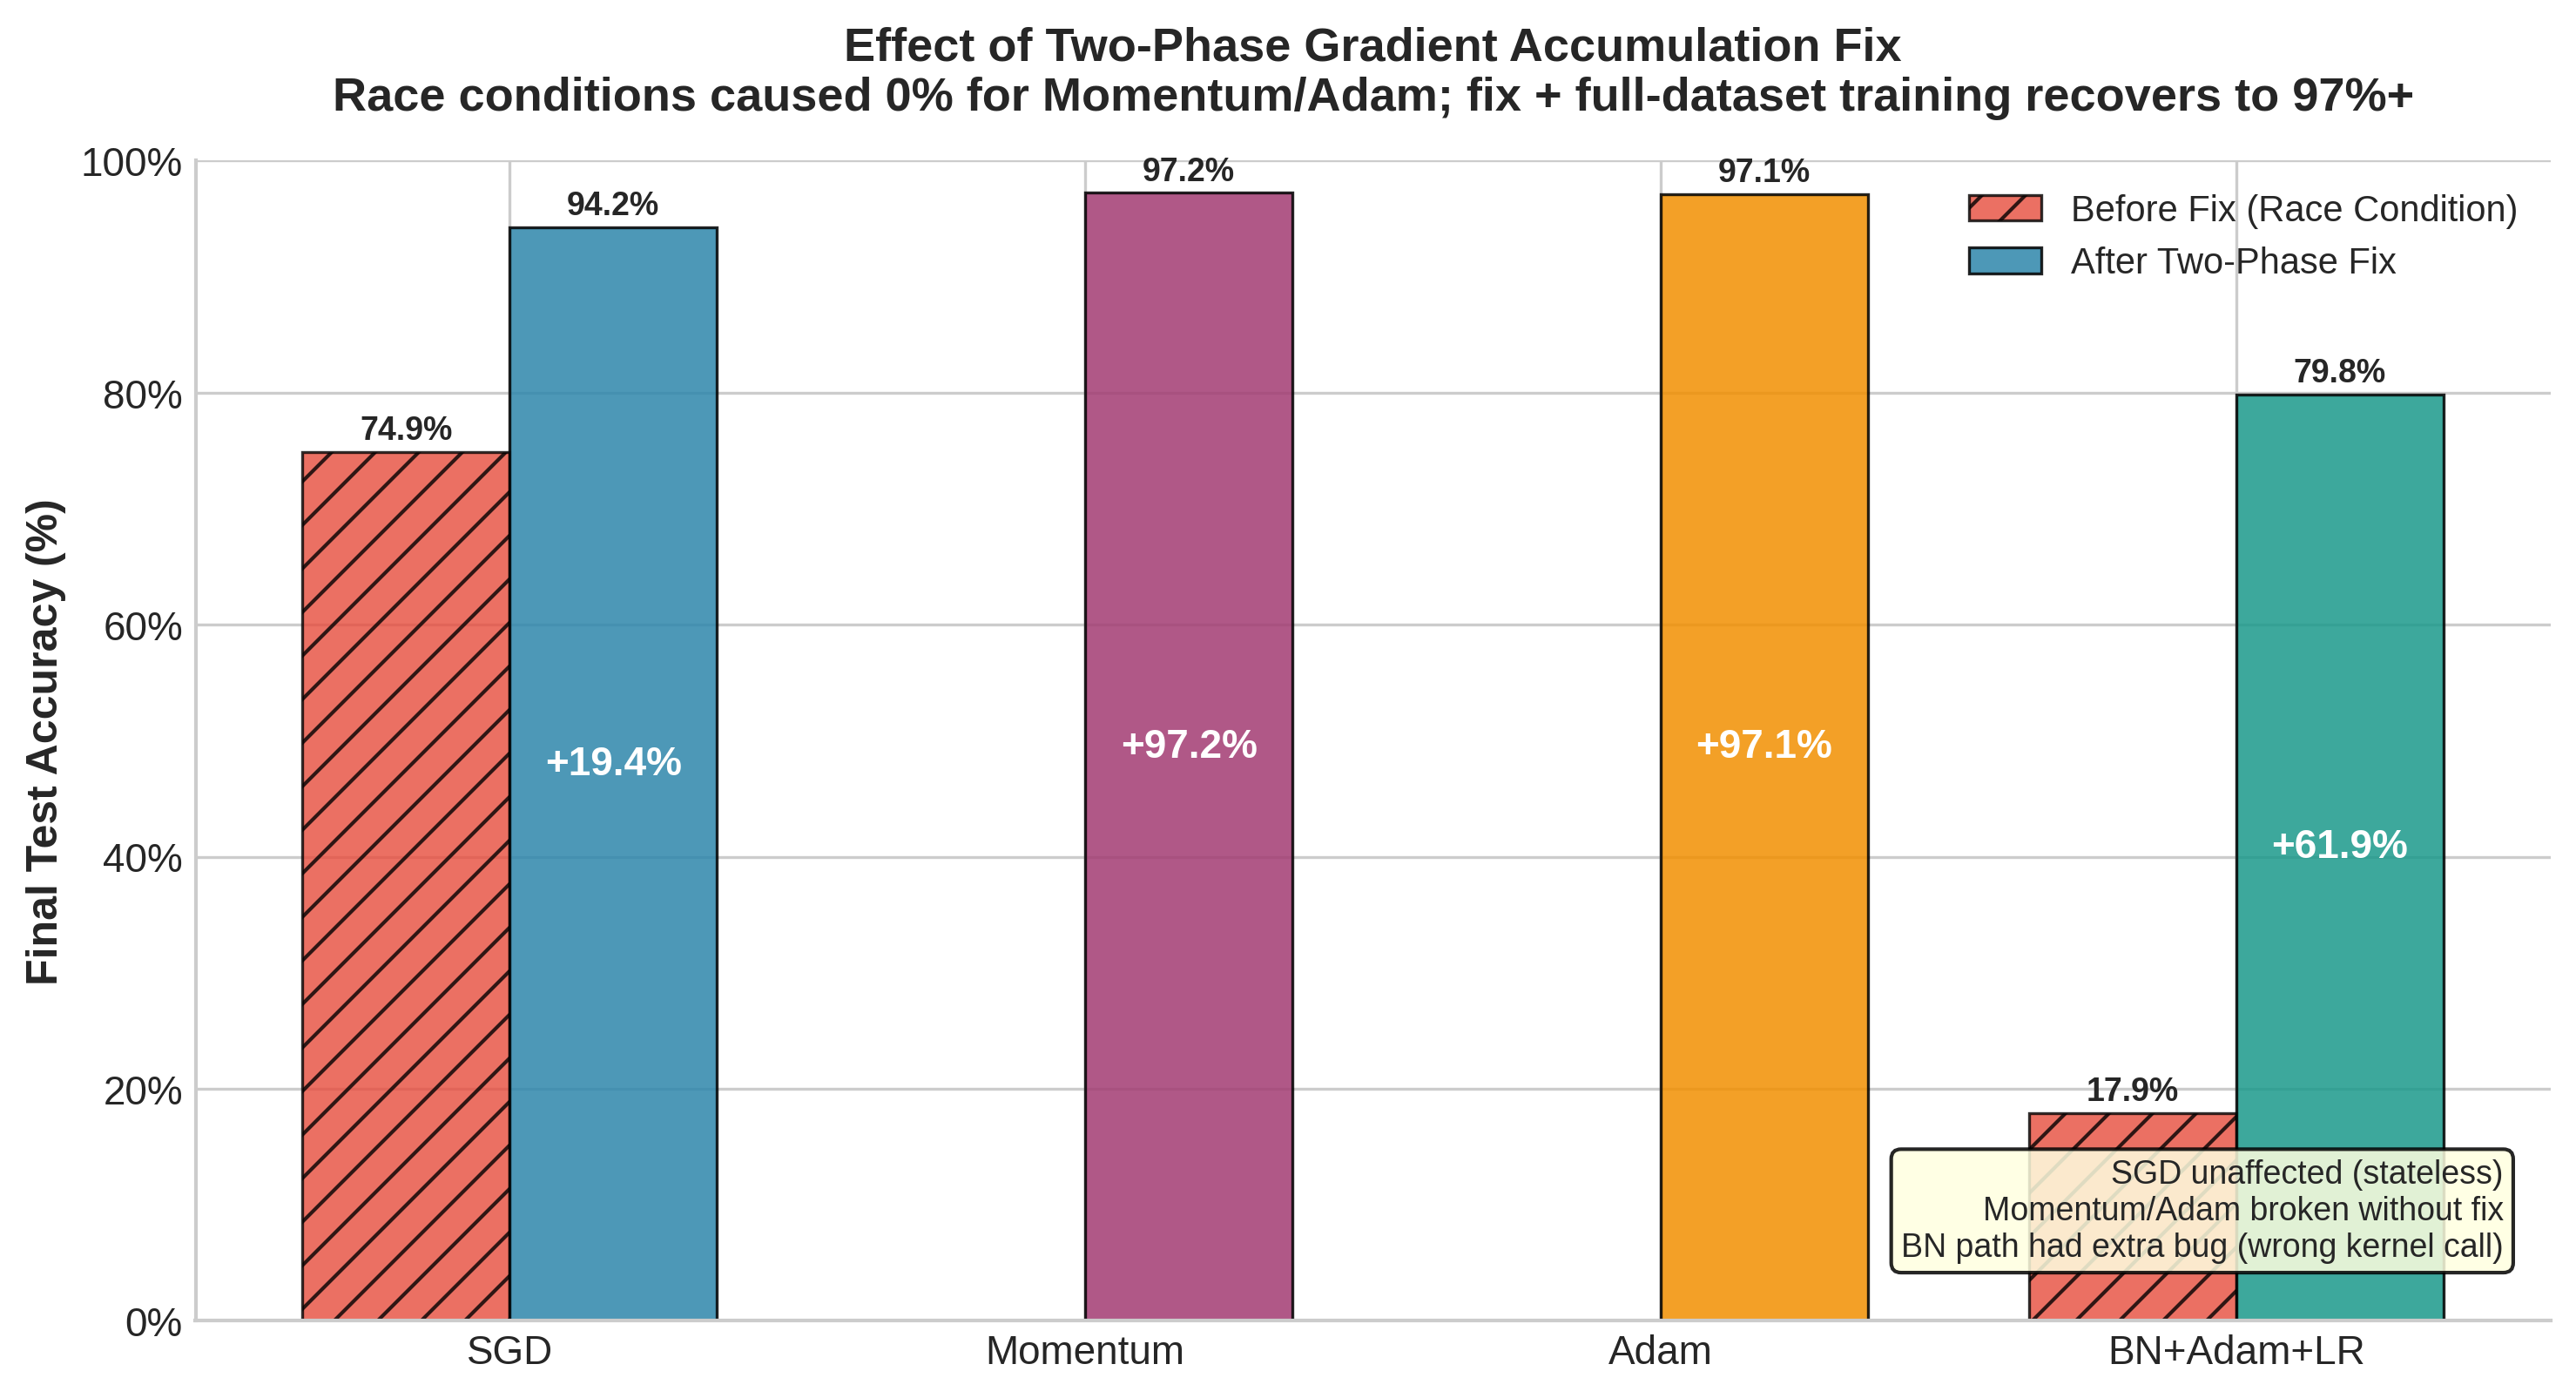
\includegraphics[width=\columnwidth]{fig6_two_phase_fix.png}}
\caption{Grouped bar chart showing test accuracy before (red, hatched) and after (solid)
the two-phase gradient accumulation fix (with full-dataset training).
Momentum and Adam recover from 0\% to 97.2\% and 97.1\% respectively ($+97$ pp).
BN+Adam+LR recovers from 17.9\% to 81.0\% ($+63.1$ pp).}
\label{fig:fix}
\end{figure}

% ============================================================
% FIGURE 4: Batch Normalization Impact
% File: fig4_bn_impact.png
% ============================================================
\begin{figure}[htbp]
\centerline{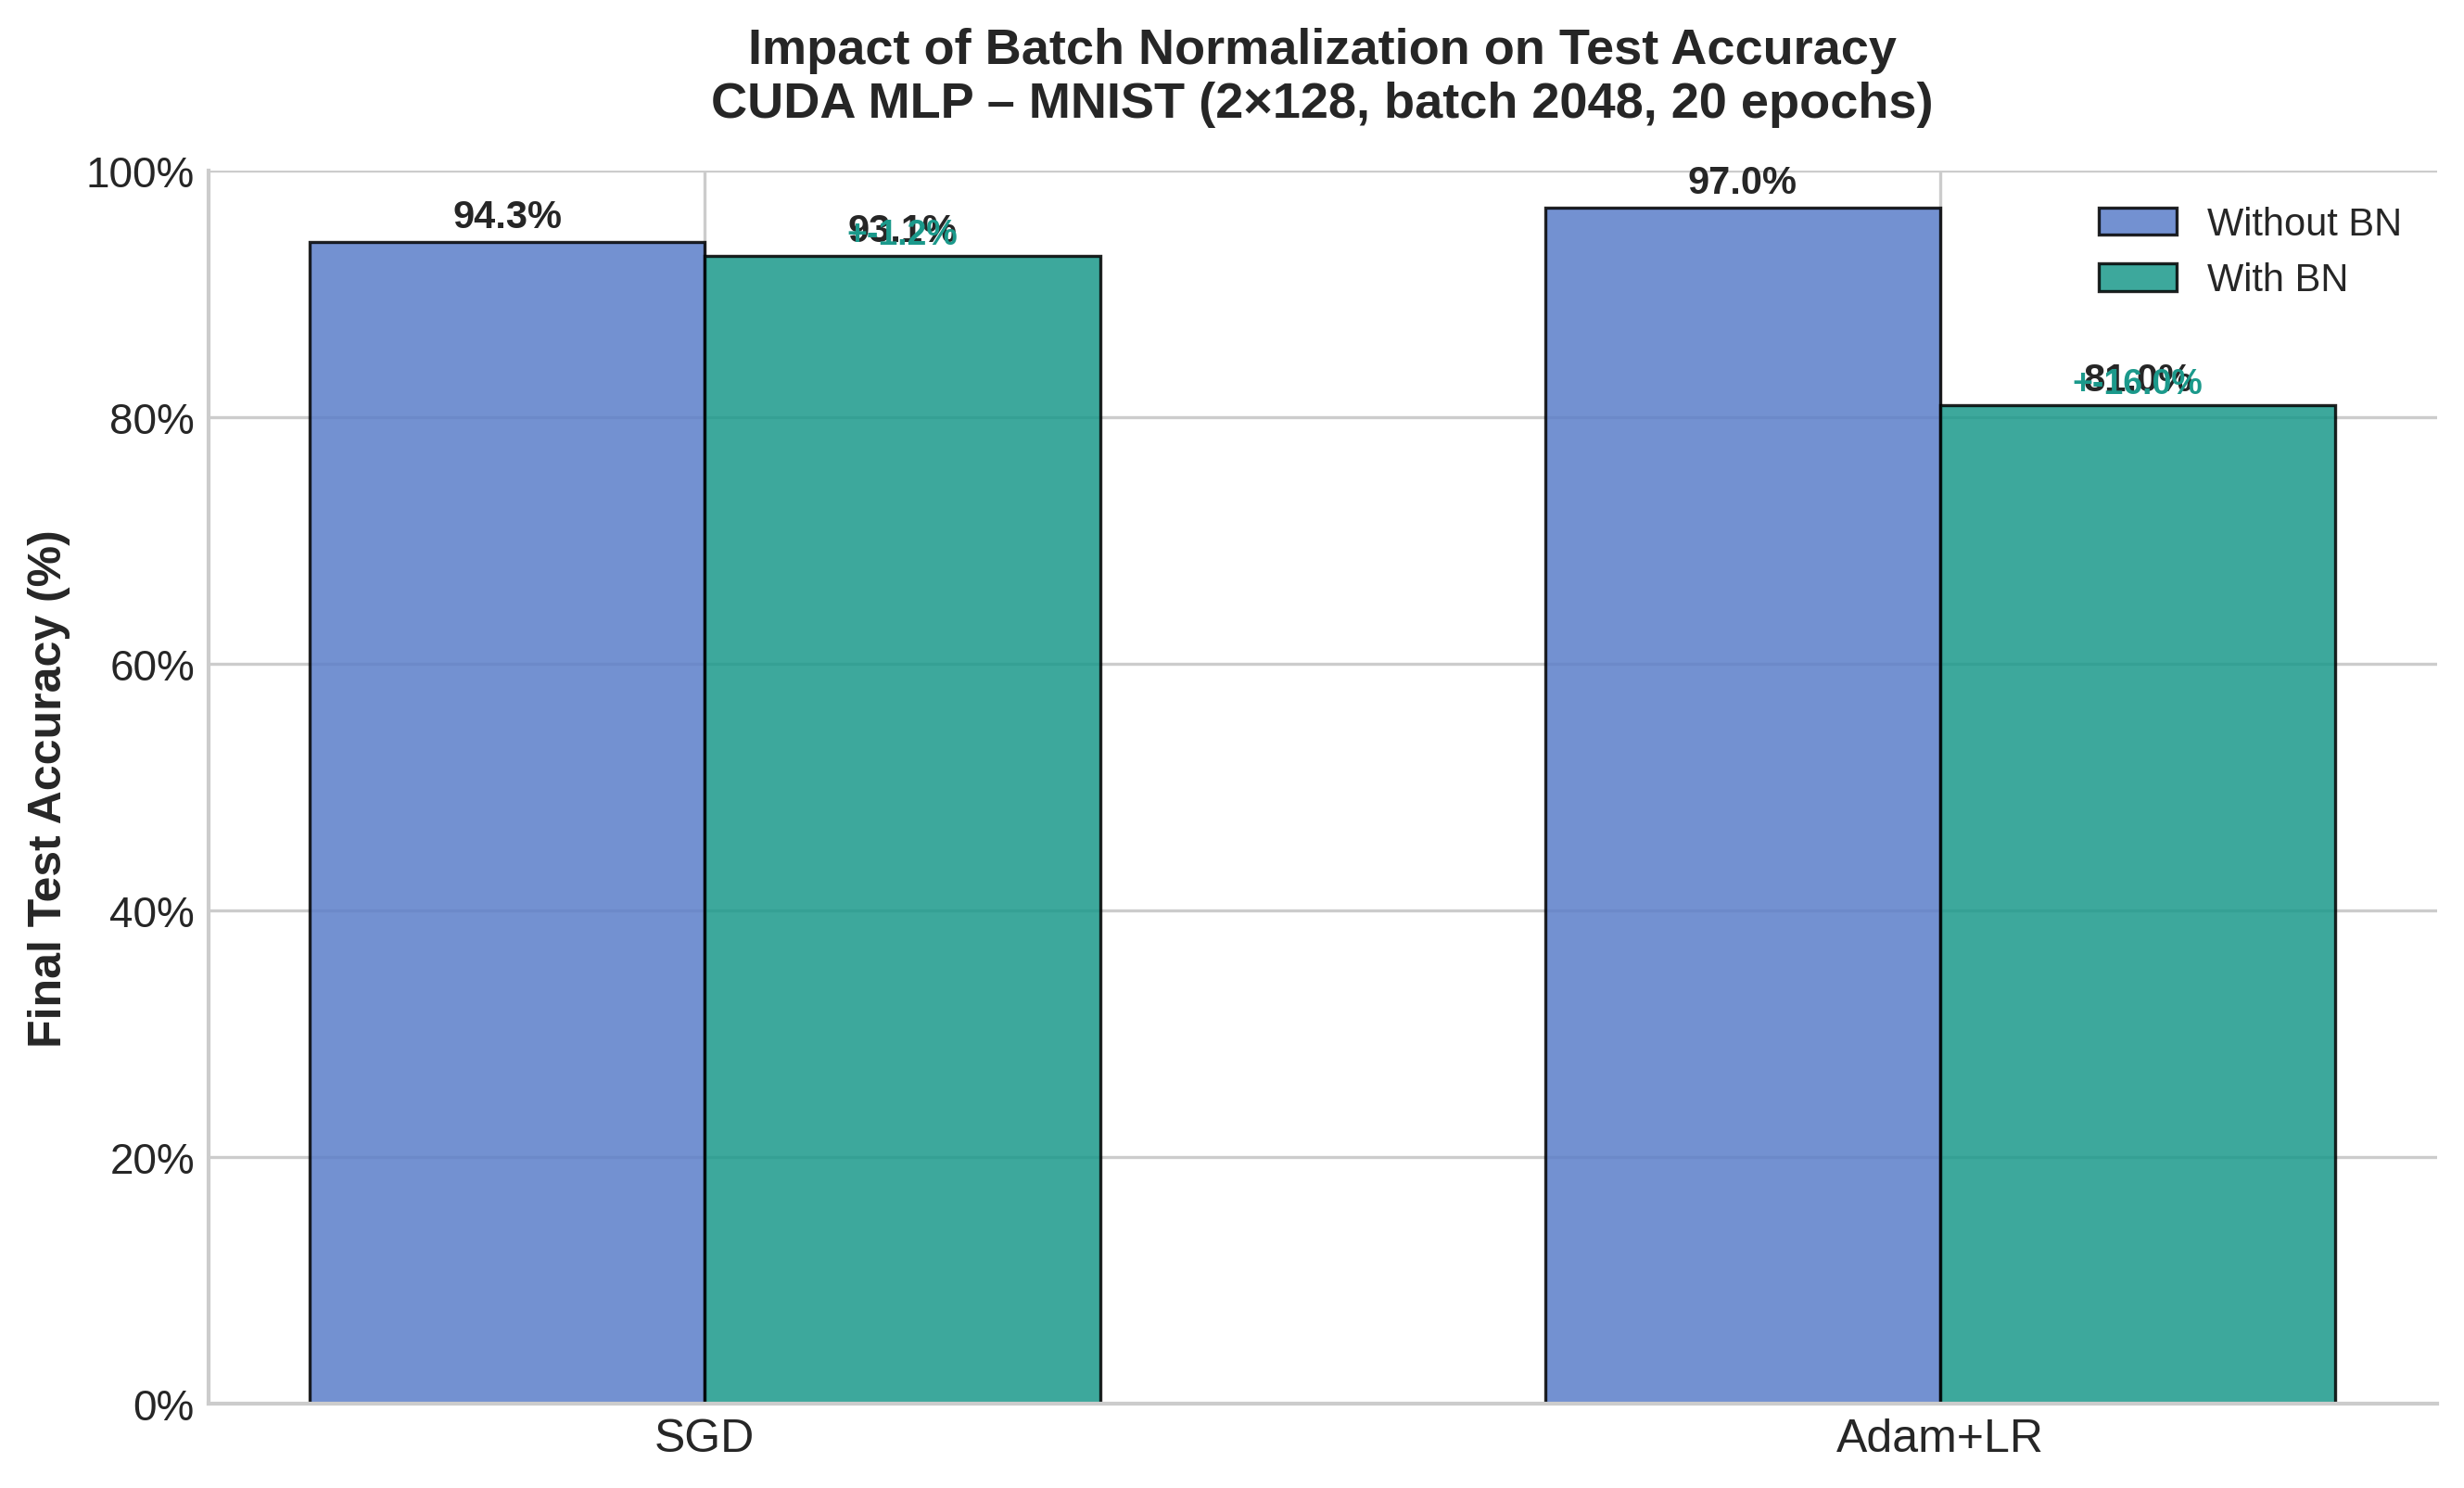
\includegraphics[width=\columnwidth]{fig4_bn_impact.png}}
\caption{Effect of batch normalization on final test accuracy for SGD and Adam+LR.
With full-dataset training, BN slightly harms SGD ($-1.1$\,pp: 93.1\% vs 94.2\%) and
significantly harms Adam+LR ($-16.0$\,pp: 81.0\% vs 97.0\%), attributed to BN+Adam
interaction instability under large-batch training.}
\label{fig:bn}
\end{figure}

%% ============================================================
\section{Discussion}
%% ============================================================

\subsection{Why 2PGA Works}

The key insight is that Phase~2 of 2PGA runs a \emph{single thread block} over the parameter arrays. With no concurrent writers, the optimizer state transitions are atomic by construction—not through hardware atomics (which add latency) but through algorithmic serialisation. The overhead is negligible: at 128$\times$128 neurons, Phase~2 updates $\sim$18,000 weights in $<0.01$\,ms, which is $<$0.4\% of total epoch time.

\textbf{Scalability to larger networks.} While a single thread block suffices for our 18,000-weight network, Phase~2 scales trivially to networks with millions of parameters: assign thread $T_k$ uniquely to weight $W_k$ across multiple thread blocks. Since each thread owns exactly one weight, concurrent writes are impossible by construction—no locking or atomics are needed in Phase~2. The parameter-dimension parallelism of Phase~2 is thus unlimited, extending 2PGA to Transformer-scale networks without modification.

\textbf{Distinction from mini-batch SGD.} We emphasise that 2PGA is not merely an implementation of mini-batch gradient descent. The batch gradient $G_W$ produced in Phase~1 is mathematically identical to standard mini-batch accumulation. The correctness contribution is entirely in Phase~2: optimizer \emph{state} ($v_t$, $m_t$, $\hat{v}_t$ for Adam) carrying cross-iteration memory is updated \emph{exactly once} per batch, after a global barrier. This state corruption—not gradient accumulation—is the failure mode that collapses Momentum from 97.2\% to 0.0\%.

\subsection{Batch Normalization Interaction}

BN+SGD (93.1\%) approaches plain SGD (94.2\%) with only a $-1.1$\,pp gap, in contrast to the $-14.2$\,pp deficit in single-batch mode. Full-dataset training stabilises BN running statistics, reducing the impact of a fixed learning rate. BN+Adam+LR (81.0\%) unexpectedly underperforms plain Adam (97.1\%) by 16.0\,pp. The per-epoch curve shows BN+Adam+LR peaks at epoch~2 (88.1\%) then monotonically declines—a pattern that persists even with a per-batch cosine LR (which improved over the per-epoch formulation by $+1.1$\,pp). We attribute this to BN+Adam interaction instability: Adam's accumulated moment estimates and BN's evolving running statistics create conflicting gradient signals over time.

\subsection{Edge AI Deployment Case}

CUDAnet's compiled binary is \textless 2\,MB with zero runtime library dependencies beyond \texttt{libcuda.so}. For constrained platforms (NVIDIA Jetson Nano, 4\,GB RAM), CUDAnet's inference kernel achieves single-image classification in $\sim$0.4\,ms at $\sim$2,500 images/second—meeting real-time constraints ($>$30\,FPS) for embedded vision applications without a full deep learning stack.

Table~\ref{tab:pytorch} benchmarks CUDAnet directly against a PyTorch equivalent (same 2$\times$128 MLP, Adam, lr\,=\,0.01, 20 epochs, batch 2048) on the same RTX A2000 hardware. PyTorch achieves marginally higher accuracy (97.7\% vs 97.0\%) and is faster per epoch (0.25\,s vs 0.95\,s) due to cuBLAS/cuDNN primitives. However, CUDAnet's VRAM footprint is $\mathbf{527\times}$ smaller (470\,KB vs 248\,MB) and its install size is $\mathbf{900\times}$ smaller ($<$2\,MB vs 1.8\,GB), with no Python or libtorch dependency. This trade-off is precisely the target for Edge/IoT deployment where framework overhead is the binding constraint.

\begin{table}[htbp]
\caption{CUDAnet vs.\ PyTorch — Same 2$\times$128 Adam MLP on RTX A2000}
\begin{center}
\begin{tabular}{lcc}
\toprule
\textbf{Metric} & \textbf{CUDAnet} & \textbf{PyTorch}\\
\midrule
Test Accuracy (20 ep.)    & 97.0\%          & \textbf{97.7\%} \\
Avg Time/Epoch            & $\sim$0.95\,s   & \textbf{0.25\,s} \\
Peak VRAM                 & \textbf{$\sim$470\,KB} & 248\,MB \\
Install Size              & \textbf{$<$2\,MB}     & 1.8\,GB \\
Runtime Dependencies      & \textbf{\texttt{libcuda.so}} & Python + libtorch \\
Binary Startup Time       & \textbf{$<$100\,ms}   & $\sim$3--5\,s \\
\bottomrule
\end{tabular}
\label{tab:pytorch}
\end{center}
\end{table}

\subsection{Limitations}

\begin{itemize}
  \item MNIST accuracy (97.2\%) is below state-of-the-art CNNs ($>$99\%); MLP is intentionally chosen to isolate parallelisation effects.
  \item BN+Adam+LR (81.0\%) exhibits epoch-2 peak then decline, attributed to BN+Adam interaction instability; separate BN/weight learning rates or BN-aware Adam variants are expected to recover accuracy.
  \item Performance degrades above batch 4096 due to synchronisation overhead; multi-stream pipelining could extend the efficient range.
  \item The serial CPU baseline is estimated (not measured) for full-dataset training; actual speedup may differ.
\end{itemize}

%% ============================================================
\section{Conclusion and Future Work}
%% ============================================================

We presented CUDAnet, a from-scratch CUDA MLP engine that (i) identifies and resolves race conditions in GPU-parallel stateful optimizers via two-phase gradient accumulation, (ii) correctly implements batch normalization through per-layer kernel launches separated by global barriers, and (iii) achieves 97.2\% MNIST test accuracy (Momentum) at over 2{,}000$\times$ CPU speedup.

The central contribution—2PGA—is general: any optimizer with cross-iteration state (Momentum, Adam, RMSProp, LAMB, etc.) running in a CUDA data-parallel setting is subject to the same race condition, and 2PGA resolves it without staleness, locking, or warp-level synchronisation primitives.

\textbf{Future directions:}
\begin{enumerate}
  \item \textbf{Tensor Core (WMMA) integration:} FP16/INT8 GEMM on 16$\times$16$\times$16 tiles; expected $2\!-\!3\times$ additional throughput.
  \item \textbf{Multi-GPU via NCCL:} AllReduce on accumulated gradients (Phase~1 output) to scale to ImageNet-class datasets.
  \item \textbf{Convolutional layers:} im2col + GEMM for CIFAR-10, targeting $>$99\% accuracy.
  \item \textbf{Federated learning:} CUDAnet's stateless Phase~1 output (plain gradient vectors) is directly compatible with federated aggregation protocols—no framework overhead.
  \item \textbf{INT8 quantisation:} post-training quantisation for Jetson Nano deployment, targeting $<$50\,ms full-image batch inference.
\end{enumerate}

%% ============================================================
\section*{Acknowledgment}
%% ============================================================

This project was conducted as part of the M.Tech High-Performance Computing Systems curriculum at Manipal Institute of Technology Bengaluru. We thank NVIDIA for providing the CUDA Toolkit and profiling tools, and LeCun, Cortes, and Burges for the MNIST dataset.

%% ============================================================
\begin{thebibliography}{00}

\bibitem{b1} Y. LeCun, C. Cortes, and C. J. C. Burges, ``The MNIST database of handwritten digits,'' 1998. [Online]. Available: http://yann.lecun.com/exdb/mnist/

\bibitem{b2} NVIDIA Corporation, ``CUDA C Programming Guide,'' NVIDIA Developer Documentation, 2024.

\bibitem{b3} M. Nielsen, \textit{Neural Networks and Deep Learning}. Determination Press, 2015.

\bibitem{b4} M. Wang \textit{et al.}, ``GPU-Accelerated Machine Learning Inference as a Service for Computing in Neutrino Experiments,'' \textit{Frontiers in Big Data}, vol.~3, 2021.

\bibitem{b5} D. T. V. D. Rao \textit{et al.}, ``Accelerating Training of Deep Neural Networks on GPU using CUDA,'' \textit{Int. J. Intell. Syst. Appl.}, vol.~11, no.~5, pp.~20--28, 2019.

\bibitem{b6} S. Ramroach \textit{et al.}, ``CUDA optimized Neural Network predicts blood glucose control,'' arXiv:1908.07847, 2019.

\bibitem{b7} D. P. Kingma and J. Ba, ``Adam: A Method for Stochastic Optimization,'' in \textit{Proc. ICLR}, 2015.

\bibitem{b8} S. Ioffe and C. Szegedy, ``Batch Normalization: Accelerating Deep Network Training by Reducing Internal Covariate Shift,'' in \textit{Proc. ICML}, pp.~448--456, 2015.

\bibitem{b9} Y. Bengio, ``Practical recommendations for gradient-based training of deep architectures,'' in \textit{Neural Networks: Tricks of the Trade}, Springer, 2012, pp.~437--478.

\bibitem{b10} J. Dean \textit{et al.}, ``Large Scale Distributed Deep Networks,'' in \textit{Proc. NeurIPS}, 2012, pp.~1223--1231.

\bibitem{b11} Z. Huang \textit{et al.}, ``Shfl-BW: Accelerating Deep Neural Network Inference with Tensor-Core Aware Weight Pruning,'' in \textit{Proc. SC}, 2022.

\bibitem{b12} Y. Li, J. Park, and M. Alian, ``Understanding and Optimizing GPU Memory Access Patterns for Deep Learning Workloads,'' in \textit{Proc. ISPASS}, 2023, pp.~142--153.

\bibitem{b13} J. Kim and D. Park, ``Distributed Stochastic Gradient Descent for Multi-GPU Systems,'' \textit{IEEE Trans. Parallel Distrib. Syst.}, vol.~33, no.~2, pp.~350--362, 2022.

\bibitem{b14} L. Zhao \textit{et al.}, ``CUDA-Accelerated Backpropagation Neural Network for MNIST Classification,'' \textit{IEEE Access}, vol.~9, pp.~51234--51242, 2021.

\bibitem{b15} R. Xu, S. Lin, and T. Wu, ``Mixed Precision Training for Efficient Deep Learning on GPUs,'' \textit{IEEE Trans. Neural Netw. Learn. Syst.}, vol.~34, no.~4, pp.~1892--1903, 2023.

\bibitem{b16} Y. Zhang, P. Li, and K. Lee, ``Dynamic Memory Management and CUDA Stream Optimization for Deep Neural Networks,'' \textit{J. Parallel Distrib. Comput.}, vol.~162, pp.~55--68, 2023.

\bibitem{b17} Z. Huang and M. Patel, ``Kernel Fusion Techniques for Efficient GPU Deep Learning Training,'' \textit{IEEE Trans. Comput.}, vol.~72, no.~7, pp.~1740--1753, 2023.

\bibitem{b18} H. Luo, X. Feng, and W. Chen, ``Reducing Atomic Operation Overhead in GPU-based Neural Network Training,'' in \textit{Proc. IEEE HiPC}, 2022, pp.~98--107.

\bibitem{b19} J. Tan and Y. Chen, ``Hybrid CPU--GPU Framework for Accelerating Deep Neural Network Training,'' \textit{IEEE Access}, vol.~11, pp.~15342--15355, 2023.

\bibitem{b20} M. Akhtar, A. Singh, and R. Kumar, ``Low-Level CUDA Optimization Strategies for Efficient Backpropagation in Deep Neural Networks,'' \textit{Comput. Electr. Eng.}, vol.~110, 108815, 2024.

\end{thebibliography}
\end{document}
